\section{Tabla hash}

\subsection{Leer un archivo que contenga los nombres de 200 animales. (revolver dichos nombres, es decir que no estén en orden alfabético)}
Para esta parte se utilizó el siguiente código:
\begin{figure}[ht]
  \centering
  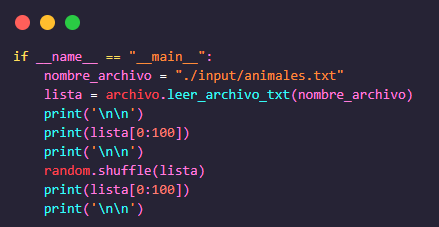
\includegraphics[width=0.7\linewidth]{./src/img/hash/codigo.png}
\end{figure}
\begin{itemize}
  \item leemos la ruta del archivo donde contiene los 200 nombres de animales.
  \item procesamos la lista para que nos regrese una lista de cada animal.
  \item desordenamos la lista de animales para que cada resultado sea diferente en cada iteracion del programa.
\end{itemize}

Resultados de la imprecion de la lista de animales primera ocacion:
\begin{figure}[ht]
  \centering
  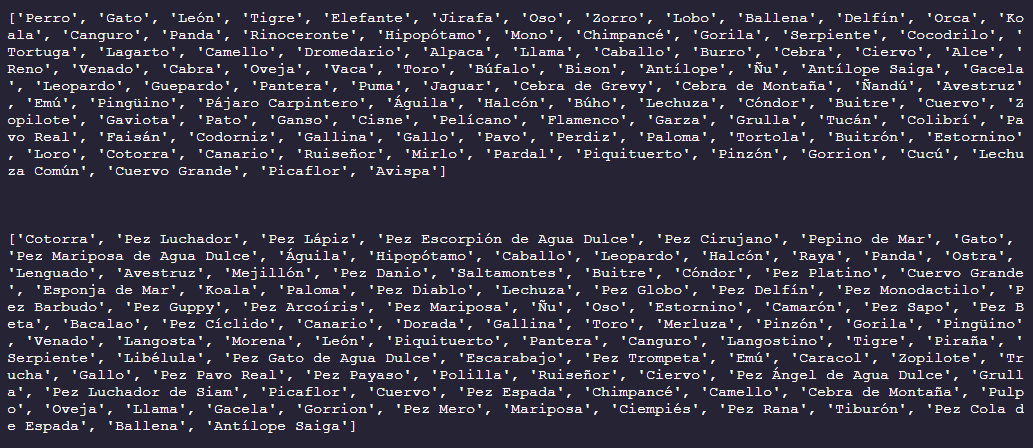
\includegraphics[width=0.7\linewidth]{./src/img/hash/image1.png}
\end{figure}

Resultado de la imprecion de la lista de animales por segunda ocacion:
\begin{figure}[ht]
  \centering
  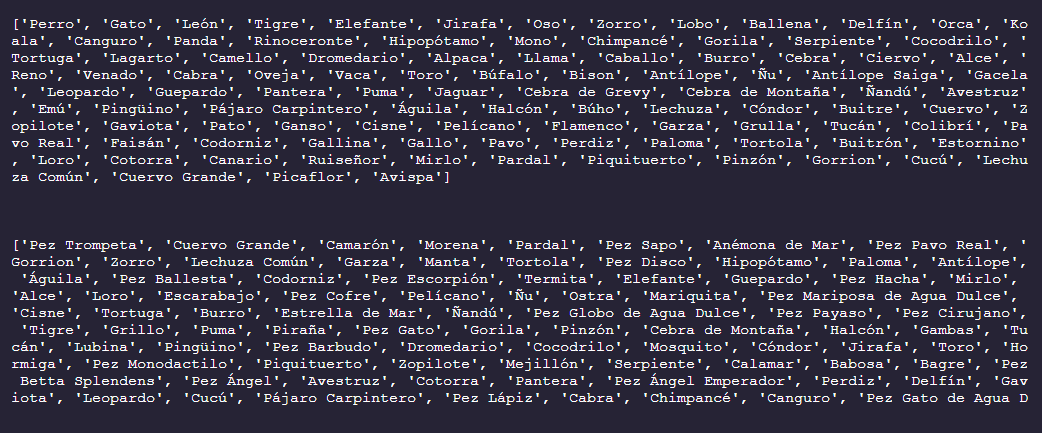
\includegraphics[width=0.7\linewidth]{./src/img/hash/image2.png}
\end{figure}

\newpage
\subsection{Investigar una función hash en python que permita asignar un valor hash a cada palabra.}
\begin{itemize}
  \item Inicialización:\newline Se define una variable hash\_val para almacenar el valor del hash.\newline Se define una lista hash\_steps para almacenar los pasos del cálculo.
  \item Recorrido de la palabra:\newline Se recorre cada carácter de la palabra (word).\newline Para cada carácter:\newline Se calcula la potencia de 2 elevada a la posición del carácter (i + 1).\newline Se multiplica el valor del caracter por la potencia de 2 y se suma al valor del hash (hash\_val).\newline Se crea una cadena que representa el paso del cálculo (paso actual):\newline Se concatena el código ASCII del caracter (ord(char)) con el símbolo "\^".\newline Se concatena la posición del caracter (i + 1) al final de la cadena.\newline Se añade la cadena que representa el paso actual a la lista hash\_steps.
  \item Cálculo de la expresión:\newline Se utiliza la función join con el caracter "+" como separador para unir todos los elementos de la lista hash\_steps.\newline La expresión formada por la concatenación de los pasos se denomina hash\_expression.
  \item Retorno:\newline Se retorna una tupla con dos elementos:\newline hash\_val: El valor del hash calculado.\newline hash\_expression: La expresión que representa los pasos del cálculo.
\end{itemize}
Ejemplo:
Considerando la palabra "Hola"
\begin{itemize}
  \item Posición 1 (H):\newline hash\_val = 72 * 1 = 72
  \item Posición 2 (o):\newline hash\_val += 111 * 2 = 294
  \item Posición 3 (l):\newline hash\_val += 108 * 3 = 702
  \item Posición 4 (a):\newline hash\_val += 97 * 4 = 1196
\end{itemize}

Resultado:
\begin{itemize}
  \item hash\_val = 2264
  \item hash\_expression = "72*1 + 111*2 + 108*3 + 97*4"
\end{itemize}

Para esto con el valor de la palabra "Hola" se obtiene el valor hash de 2264 y la expresión que representa los pasos del cálculo es "72*1 + 111*2 + 108*3 + 97*4".\newline Ahora se saca el modulo del valor para que el valor sea menor a 200 y el modulo sea el valor hash que se le asignara a la palabra y su respectiva celda en la tabla hash.

\begin{figure}[ht]
  \centering
  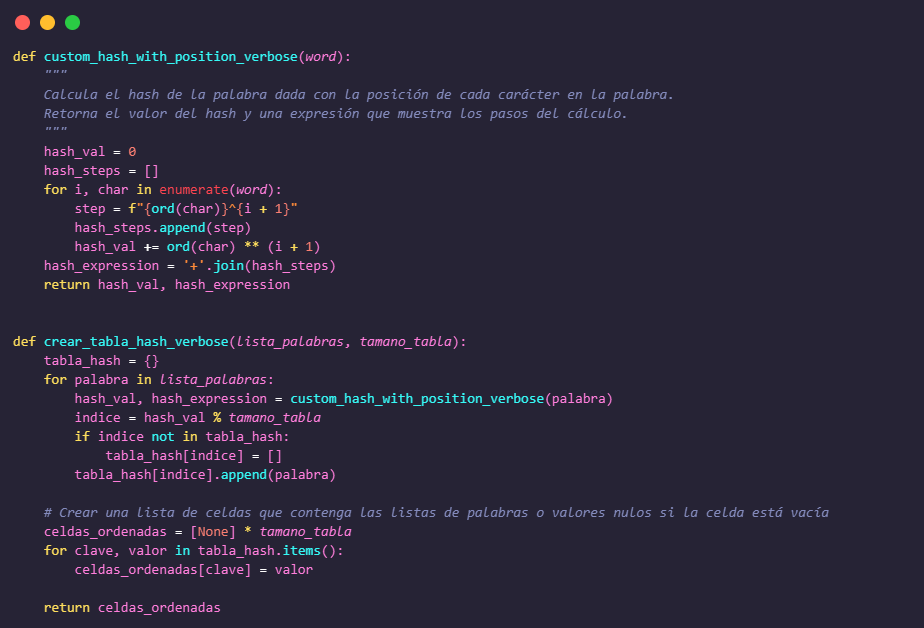
\includegraphics[width=0.7\linewidth]{./src/img/hash/image3.png}
\end{figure}

\newpage
\subsection{Insertar cada nombre de animal en una misma tabla hash}

Para esta parte, mostramos la lista de la tabla hash con los nombres de los animales.\newline Para cada palabra:\newline Se calcula el valor del hash y la expresión del hash utilizando la función custom\_hash\_with\_position\_verbose.\newline Se calcula el índice de la celda en la tabla hash utilizando el módulo (hash\_val \% tamano\_tabla).

\begin{figure}[ht]
  \centering
  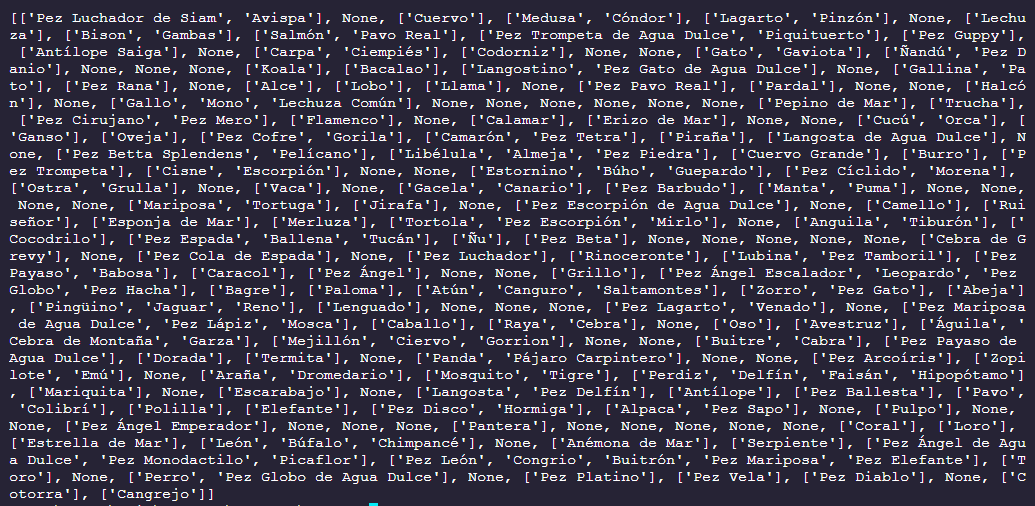
\includegraphics[width=0.7\linewidth]{./src/img/hash/image4.png}
\end{figure}


\subsection{Mostrar la lista de animales con sus respectivos valores hash}

Mostramos en una tabla el indice que se le asigno a cada animal en su respectiba celda de la tabla hash aunque hay coliciones en la tabla hash.

\begin{figure}[ht]
  \centering
  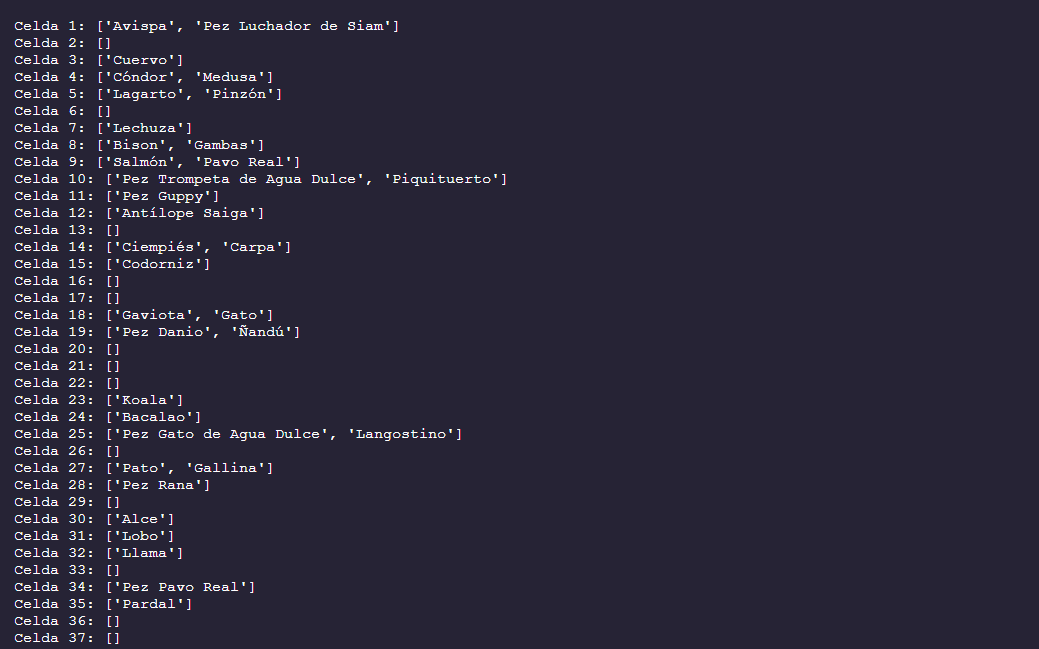
\includegraphics[width=0.6\linewidth]{./src/img/hash/image5.png}
\end{figure}

\newpage
\subsection{Realizar una consulta al árbol sobre una palabra que sí exista y otra que no exista y mostrar los resultados}

Para esta parte ingresamos dos palabras una con el nombre de un animal y otra con nombre de una persona. La primera palabra si existe en la tabla hash y la segunda no existe en la tabla hash. 

\begin{figure}[ht]
  \centering
  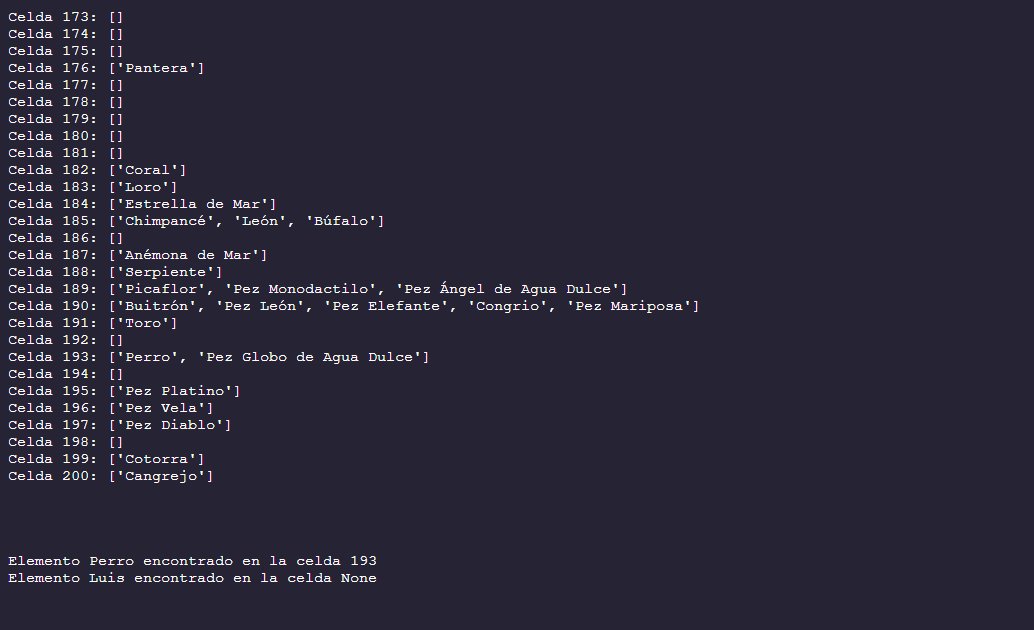
\includegraphics[width=0.6\linewidth]{./src/img/hash/image6.png}
\end{figure}

para esta parte en ves de buscar por toda la tabla hash lo que se hace es hacer el procesamiento hash de la palabra y buscar en la celda que le corresponde a la palabra en la tabla hash.

\begin{figure}[ht]
  \centering
  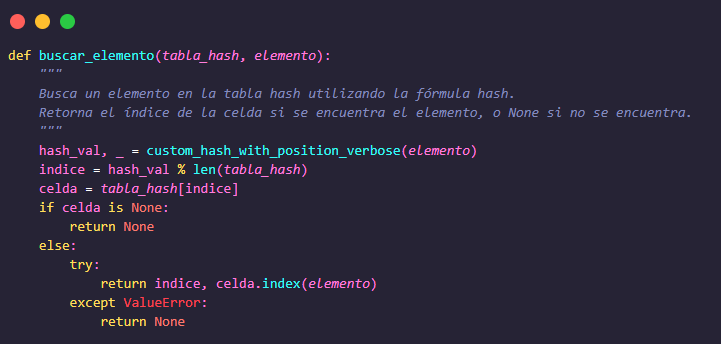
\includegraphics[width=0.6\linewidth]{./src/img/hash/image7.png}
\end{figure}